\documentclass[]{report}   % list options between brackets
\usepackage{graphicx, url, placeins, algorithm, algorithmic, hyperref, lipsum, cite, caption, subcaption}
\graphicspath{{figures/}}

\begin{document}

\title{Monte Carlo-based ray tracer\\ Project Report}   % type title between braces
\author{
	Johan Beck Nor\'{e}n, johbe559@student.liu.se
	\\Andreas Valter , andva287@student.liu.se
	}
\date{\today}    % type date between braces
\maketitle

\setcounter{page}{2}
\chapter{Abstract}
\emph{ A brief and concise summary of the article. It should be limited to 1000 characters.}
\chapter{Introduction}
Realistic lighting in computer graphics scenes has been a problem for many years.
\emph{You should describe here global lighting models and talk about Whitted ray tracing, radiosity, Monte Carlo ray-tracing, two-pass rendering, photon mapping and ray-tracing of isosurfaces, explaining how they work and what they do. 
This description should be done mainly in words and not so much with maths. 
Also do not go too much into detail. 
The explanations should be done with the help of the papers above that were presented during the seminar. 
You should reference these papers in the introduction. 
The introduction is concluded by a paragraph, that describes the structure of the paper like: "The first section is the introduction. 
In section 2, we discuss in more detail the techniques regarding (raytracing, Monte Carlo raytracing, depending on what you have implemented), which we have implemented. 
Section 3 shows some results that we have obtained with our implementation and benchmarks. 
The discussion and the outlook is the section 4." 
Length: about 3 pages.}

\begin{equation} \label{eq:light}
A=B
\end{equation}

\section{Global lightning}


\section{Whitted ray tracing}
The Whitted ray tracing method described by Turner Whitted in \cite{} was the first global illumination method that took the whole scene into consideration when calculating intensity values.
In previous so called ray marching solutions, the calculations stopped as a ray hit a surface and local lightning models like Lambert's cosine rule to model perfectly diffuser or the Phong model. \\

\begin{equation} \label{eq:phong}
\emph{I} = \emph{I}_{a} + \emph{k}_{d} \sum_{j=1}^{j=ls} (  \bar{N} .  \bar{L}_j) + \emph{k}_{s} \sum_{j=1}^{j=ls} (  \bar{R}_j .  \bar{V})^n
\end{equation}

The Phong model given by \autoref{eq:phong} is a local light model.
It assumes that each light source $\emph{L}_j$ is located at a point with infinite distance to the objects in the scene. 
The total reflected intensity $\emph{I}$ is calculated using the reflection due to ambient light $\emph{I}_{a}$ together with two terms, one term for diffuse light and one specular term.
The two constants $\emph{k}_{d}$ and $\emph{k}_{s}$ is reflection constants that regulates their contributions.
The diffuse term uses the Lamberts cosine law to describe the color using a dot product between the normal and the light direction to calculate if that part of the surface is directed towards the light source.

The specular term uses the direction that a perfect reflection $ \bar{V} $ from the light source would take on the surface together with a ray towards the viewer $\bar{V}$.\\

Whitted extended the previous techniques and allowed for rays to bounce in the scene and thus creating the basis for global illumination.
The solution he presented allowed for true reflections, shadows and refractions.
By using the Phong model on each ray hit and spawning new rays recursively for reflections, shadow rays and refractions a method for simulating global lightning is created.

\section{Radiosity}
Radiosity is an algorithm for global illumination which only handles diffusely reflected light, and is therefore not dependent on any camera position or direction.
This means that the solution converges toward a steady state, and can for example be pre-computed for use in static scenes.
The algorithm works by splitting the scene geometry into a number of finite area elements called patches, and solves the rendering equation for surfaces that diffusely reflects light.
A visibility factor, called \emph{form factor}, is used to describe a patch's visibility toward all other patches in the scene.
The size of a view factor is dependent on the distance between any two patches, their orientation in relation to each other, partial or total occlusion etc. and describes the amount of radiance leaving a patch $j$ arriving at patch $i$ for all patches $j \in N$ for a scene consisting of $N$ number of patches.
The form factors make up a system of linear equations, which when solved produces the radiosity for each patch.
The process can be iterated to perform several passes and allowing for multiple bounces to be computed.

\section{Monte Carlo ray tracing}
A rendering equation (\autoref{eq:rendering_eq}) presented by Kajiya in \cite{kajiya} describes a full global illumination solution for a given scene.
It is an integral equation called a Fredholm equation of the second kind because of the unknown radiance quantity, $L(...)$, appears on both sides of the equation.
This makes the equation a recursive one, corresponding to a ray's multiple bounces through a scene.
It is described below using the same notation as Dutr\'{e} et al. in \cite{dutre}, and we will use this notation throughout this report.
\begin{equation}
\label{eq:rendering_eq}
L(x \rightarrow \theta) = L_e(x \rightarrow \theta) + \int_{\Omega_x} f_r(x, \Phi \rightarrow \theta)L(x \leftarrow \Phi)cos(N_x, \Phi)d\omega_{\Phi}
\end{equation}
The Monte Carlo integration method introduces a method for calculating an estimated value for an integral expression.
This is done by sampling the integral function by random discreet numbers, and as the number of samples increase the produced solution's accuracy increases as well.
Similar to a Whitted ray tracer, a Monte Carlo ray tracer starts by shooting rays from a virtual camera through a view plane into the scene.
One difference is that Monte Carlo ray tracing handles diffuse and specular surface inter-reflections, diffuse reflections, color bleeding between objects, and soft shadows by stochastically sampling area light source surfaces for each ray intersection.
As the number of samples increase the more accurate to integral estimation will be, and the algorithm produces noise if the number of samples are too low.
There are several ways to reduce the noise.
One could separate the calculations for direct and indirect illumination, using shadow rays to more quickly compute direct diffuse illumination and soft shadows.
Sampling directions for diffuse indirect illumination could be chosen in more informed ways to reduce the noise.
There have also been research on methods combining the benefits of radiosity with the benefits of ray tracing.

\section{Two-pass rendering}
Since a radiosity method handles diffuse reflections rather well, and a ray tracing method handles specular reflections well. a lot of research has been done to find ways to combine these two methods.
One of these methods descibed by Smits et al. \cite{importance_radiosity} works from the fact that radiosity algorithms propagate light from a light source through the scene, while a ray tracing algorithm only cares about the light that reaches the eye.
The method in \cite{importance_radiosity} consists of splitting the rendering into two passes.
The first pass uses a ray tracing approach to emmit importance from the eye through the scene.
This importance is then used to refine the patches used for the second pass, a radiosity pass.
By subdividing patches in parts with high importance, and ignoring patches in areas with little or no importance, great speedups can be achieved.

\section{Photon mapping}
Monte carlo methods for ray tracing suffers from noise in the final results if not enough samples are used when calculating radiance from diffuse indirect illumination.
Photon mapping is two-pass global illumination method presented by Jensen \cite{photon_maps} which computes diffuse indirect illumination faster than a Monte Carlo solution.
The method works by emitting packets of energt (light) from the light sources toward different objects in the scene.
Different packets can be used for different materials, e.g. a high resolution photon map can be used for caustics that are visualized directly, while a lower resolution map can be stored for later use in the ray tracing step.
Shadow photons can be used to more efficiently compute shadows, and be used as directional information to produce more accurate sampling directions during the rendering step.
The method has been shown to reduce rendering time as well as the noise in the final image when used in a Monte Carlo ray tracer algorithm.

\section{Iso surface ray tracing}
An iso surface is a surface described implicitly by a mathematical expression or equation.
An iso surface representation of a scene is preferable over polygonal objects in a ray tracing context for a few reasons.
Implicitly described primitives and objects usually scale well if the resolution or precision of the illumination algorithm should increase, since they are not bound by a finite number of triangles, but rather a mathematical description.
They are also easy to define and describe, and are rather straight-forward to calculate ray intersections against.
From an intersection calculation we need to decide weather a ray is intersecting the surface, and if so at what position, and what is the normal vector for the surface at that position.
Different data structures can be used to greatly increase the performace of intersection tests, such as storing surfaces in an \emph{octree} structure or using a \emph{bounding volume hierarchy} (BVH).

\section{Report structure}
The first chapter is an introduction to global illumination.
In chapter 2 we will go into more detail regarding the techniques mentioned in chapter 1 that we have implemented.
Chapter 3 will present our results from our implementation along with some benchmarks using different parameters, and lastly in chapter 4 a discussion about our results is presented.

\chapter{Background}
\emph{Here you describe the techniques you use in your code. 
Describe how you do ray-surface intersections, how you launch reflected and refracted rays, how you compute the intensities, what are shadow rays, etc. No C++ code. 
You may use pseudocode, but it is better do discuss the techniques only from a theoretical point of view. 
These descriptions should be accompanied by figures. 
The figures are numbered consecutively in order of appearance. 
Each figure must have a caption with a brief description of what you see in it. 
The figures must be referred to from the text and described and interpreted in more detail in the text.
Length: about 5-6 pages.}

\section{Scene storage}
When calculating global lightning for the scene, all objects need to be taken into consideration when calculating the illumination for one part of the scene due to the recursive nature of \autoref{eq:rendering_eq}.
For ray tracing solutions, this means that as rays bounce inside the scene, the first intersecting object needs to be located.
A na\"{\i}ve solution would be to store all objects without any information about where in the scene they are located.
When traversing a ray through the scene, the algorithm would have to check against all objects, even if almost all of the checks would be misses.
For a simple scene with only a few implicit objects this is a good solution. The overhead when dealing with an more complex storage method would make it slower.
But when using a more complex scene consisting of models with hundreds of thousands of elements, it is possible to take advantage of the spatial information of each element to subtract a small subset and only do collision tests against those.
There are several methods for storing the scene using different techniques.

\subsection{Bounding box}
An axis aligned bounding box is a crucial part of most scene storage methods.
This is the smallest box with axes aligned to the Cartesian coordinates axes that can encapsulate the primitive that owns the bounding box.
The bounding box will not be the smallest box that can encapsulate the primitive but the intersection tests is much simpler compared to doing collision tests against arbitrarily rotated primitives.

\subsection{Bounding volume hierarchy}
Bounding volume hierarchy (BVH) uses a tree structure with bounding volumes like axis aligned bounding boxes. 
Small sets of primitives are divided into different bounding volumes.
These small volumes are then combined to larger bounding volumes recursively until there is only one bounding volume left surrounding the entire scene.
By using this technique, it is known that if the ray does not intersect a larger bounding box, the child boxes within that larger box can be ignored as well.

\subsection{Octree}
The octree method uses the bounding boxes in a slightly different way than described in the previous section.
The scene is encapsulated into a large bounding box.
When each primitive is added, the scene bounding box is subdivided into eight sub-volumes recursively until the current level of bounding boxes are to small to fit the primitive.
The primitive is then added to the level above that as a leaf.
Using this structure, it is possible to traverse the ray through the volume and, just as when using the BVH tree, large parts of the tree can be ignored by checking only parent nodes for intersection.

\section{Intersection}
The implementation needs to be able to handle several different intersection algorithms, one for each type of primitive in the scene.
To make sure that all kinds of primitives are supported, inheritance is used where each primitive inherits from an abstract class.
During rendering calculation, the ray tracer calls an abstract method for calculation of intersection points on the given primitive and therefore the implementation supports all primitives that can define a intersection method.
Each of these methods uses an incoming ray with a direction vector $d$ and a origin $o$ described by \autoref{eq:ray}.

\begin{equation} \label{eq:ray}
\mathbf{p} = \mathbf{o} + t \mathbf{d}, t \leq 0
\end{equation}

\subsection{Implicit sphere}
A sphere is defined by a position vector $c$ of its centre and a radius scalar $r$. The goal is to find if any $t$ in \autoref{eq:ray} satisfies \autoref{eq:sphere}. By inserting \autoref{eq:ray} into \autoref{eq:sphere}, we receive an expression for solving the intersection point described by \autoref{eq:sphereray}.
\begin{equation} \label{eq:sphere}
(\mathbf{p} - \mathbf{c}).(\mathbf{p} - \mathbf{c}) = r^2
\end{equation}

\begin{equation} \label{eq:sphereray}
(\mathbf{d} . \mathbf{d})t^2 + 2(\mathbf{o} - \mathbf{c}) * \mathbf{d} t + (\mathbf{o} - \mathbf{c}) . (\mathbf{o} - \mathbf{c}) - r^2=0
\end{equation}
 
\subsection{Axis aligned bounding box}
\subsection{Quadrilateral}
\subsection{Triangle}
\subsection{Octree}

\section{Anti-aliasing by sub-pixel sampling}
To reduce aliasing effects in the final image we have implemented support for sub-pixel sampling. This means that instead of sending one view ray from the virtual camera through the center of a pixel on the view plane, we send several view rays distributed on the pixel and average their results. The view ray distribution on the pixel area can be done uniformly or by using random numbers to place them stochastically. For all renders in this report, the stochastic distribution was used. In  \autoref{fig:antialiasing} we se a comparison between using 1 view ray per pixel on the left, and 10 view rays per pixel on the right.

\begin{figure}
        \centering
        \begin{subfigure}[b]{0.3\textwidth}
                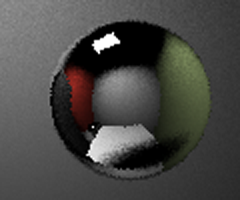
\includegraphics[width=\textwidth]{figures/aliasing_1.png}
                \caption{1 view ray per pixel}
                \label{fig:gull}
        \end{subfigure}%
        ~ %add desired spacing between images, e. g. ~, \quad, \qquad etc.
          %(or a blank line to force the subfigure onto a new line)
        \begin{subfigure}[b]{0.3\textwidth}
                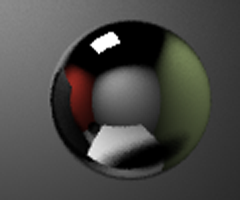
\includegraphics[width=\textwidth]{figures/aliasing_10.png}
                \caption{10 view rays per pixel}
                \label{fig:tiger}
        \end{subfigure}
        \caption{Antialising by randomly distributed sub-pixel sampling}\label{fig:antialiasing}
\end{figure}

\section{Ray tracing}
\subsection{Reflection}
\subsection{Refraction}
\subsection{Intensity calculations}
\subsection{Shadow rays}

\chapter{Results and benchmarks}
\emph{Here you show results obtained with your code. You can do series of computations, where you vary the pixel resolution, the number of ray iterations, the number and type of the objects in the scene (transparent vs opaque) etc. You can compare in detail images computed from the same scene with different resolutions. You can discuss figures and effects in the figures, like color bleeding, noise, aliasing artifacts etc. You can list benchmarks (e.g. how long it took your computer to calculate a frame with a given resolution) in a table etc. Here you can be creative and look at things you like. 
Length: about 5-6 pages .}


\chapter{Discussion}
\emph{Here you should repeat the key findings of your article and discuss how you could improve them. 
Do not go into details, but just give a general description. 
Do not use bullet points. 
You can also give an outlook on how your renderer could be improved etc. 
Length: about 1 page .}

\bibliographystyle{abbrv}
\bibliography{bibl}

\end{document}